\begin{titlepage}
\centering
\vspace*{2cm}
{\LARGE\bfseries Projet de Fin d'\'Etudes\\[0.5em]
Non-Invasive Glucose Monitoring Using\\
Transformer Models on Zybo Z7-20 FPGA\par}
\vspace{1.5cm}
{\Large\bfseries Part I: Invasive Glucose Monitoring Methods ---\\
Clinical Evidence, Accuracy Statistics, and Limitations\par}
\vspace{2cm}
{\large A systematic review of the five principal invasive techniques
currently used in clinical practice and personal diabetes management,
with quantitative analysis of their accuracy, cost, patient burden,
and fundamental barriers to continuous non-invasive deployment.\par}
\vspace{3cm}
{\large\itshape Submitted in partial fulfillment of the requirements
for the degree of Engineering\\[0.5em]
Academic Year 2024--2025\par}
\vfill
\end{titlepage}

\tableofcontents
\newpage

\chapter*{Preamble to Part I}
\addcontentsline{toc}{chapter}{Preamble to Part I}

Measuring blood glucose accurately is not a solved problem. Decades of clinical research, engineering investment, and patient suffering have produced methods that work --- but each of them extracts a cost, whether measured in drops of blood, chronic inflammation, missed hypoglycaemic episodes, or the quiet arithmetic of annual out-of-pocket spending that pushes many patients to ration their own testing.

Part I of this report examines the five principal invasive glucose monitoring methods in clinical use today: fingerstick capillary blood glucose monitoring, continuous glucose monitoring via subcutaneous interstitial fluid sensors, intravenous and venous laboratory glucose measurement, urine glucose testing, and alternative-site testing at the forearm, thigh, and palm. For each method, we present a detailed technical description, the step-by-step measurement procedure, quantified clinical performance statistics drawn from peer-reviewed trials, and --- the main focus --- a rigorous account of their limitations. The purpose is not merely to catalogue shortcomings but to build the evidentiary case for a fundamental rethinking of how glucose monitoring should work.

The statistics cited throughout this chapter come from published clinical trials and regulatory accuracy studies. Where MARD figures are stated, they correspond to the specific study populations and conditions defined in each cited work; no values have been invented or estimated.

%=============================================================
\chapter{Fingerstick Capillary Blood Glucose Monitoring}
\label{ch:fingerstick}
%=============================================================

\section{Technical Description}

Self-monitoring of blood glucose (SMBG) by fingerstick --- a lancet-based puncture of the fingertip followed by electrochemical analysis of a capillary blood drop --- has been the dominant method of point-of-care glucose measurement since the early 1970s. The technique relies on two distinct physical components: the lancing device and the reagent test strip inserted into a glucometer. Together they form a system that is deceptively simple on the surface but technically intricate underneath, with multiple layers of chemistry, calibration, and human-factors engineering whose failures translate directly into patient harm.

\subsection*{The Lancing Device and Capillary Blood Collection}

A lancing device holds a sterile lancet, typically a 28--33~gauge needle between 1.0 and 2.4~mm in length. When activated, a spring mechanism drives the lancet through the epidermis and into the dermal capillary bed of the fingertip. The fingertip is chosen because it has an  rich capillary network fed by arteriovenous anastomoses, providing rapid and reproducible access to blood that closely reflects circulating plasma glucose. Depth settings on modern devices allow adjustment for skin thickness, with shallower penetration associated with lower pain but sometimes insufficient blood volume.

The lancet punctures to a depth of roughly 0.8--1.5~mm, reaching the rete subpapillae, the superficial vascular plexus of the papillary dermis. Blood is expressed by gentle pressure, and a drop of approximately 1--3~$\mu$L is drawn onto or into the end of the test strip by capillary action. Most modern strips require only 0.3--1.0~$\mu$L of whole blood.

\subsection*{Electrochemical Transduction in Test Strips}

The majority of test strips sold today use amperometric or coulometric electrochemical detection rather than the older reflectance photometry approach. Within the strip, glucose in the blood sample reacts with an enzyme --- glucose oxidase (GOx) or glucose dehydrogenase (GDH) --- immobilised on a working electrode. The enzymatic reaction produces a current proportional to glucose concentration:

\begin{align}
\text{Glucose} + O_2 &\xrightarrow{\text{GOx}} \text{Gluconolactone} + H_2O_2 \\
H_2O_2 &\rightarrow 2H^+ + O_2 + 2e^- \quad (\text{amperometric detection})
\end{align}

The glucometer measures the current and converts it to a glucose concentration using factory-stored calibration curves. Modern meters complete this in 3--5~seconds.

A critical distinction is between whole-blood and plasma-equivalent readings. Plasma contains a higher glucose concentration than whole blood because red blood cells have lower glucose content. Early meters reported whole-blood values, approximately 11--15\% lower than plasma values at the same haematocrit. Contemporary devices are calibrated to report plasma-equivalent results, aligned with laboratory reference methods, but the underlying measurement is still made on whole blood. Haematocrit directly affects apparent glucose concentration. At abnormally low haematocrit (severe anaemia), glucose oxidase-based meters can overestimate glucose by as much as 10--15\%; at high haematocrit, the reverse bias applies~\cite{freckmann2022mard}.

\subsection*{Enzyme Selectivity and Interference}

Glucose oxidase is highly selective for D-glucose but sensitive to oxygen tension. In hypoxic patients --- including those with respiratory failure, severe peripheral vascular disease, or carbon monoxide poisoning --- reduced pO$_2$ at the fingertip can alter the amperometric signal and yield erroneously high glucose readings. Glucose dehydrogenase-based strips avoid oxygen dependence but certain formulations using GDH-pyrroloquinoline quinone (GDH-PQQ) can cross-react with galactose, maltose, and xylose. These substances are present in patients receiving peritoneal dialysis or certain intravenous solutions, making specific strip formulations dangerous in those populations.

\subsection*{Calibration and Strip Coding}

Each batch of test strips is manufactured with a specific enzyme loading, electrode geometry, and coating. Batch-to-batch variation necessitates calibration, historically performed by inserting a code chip corresponding to the strip lot. Modern systems use automatic coding via a chip embedded in the strip, eliminating one source of human error. Factory calibration is traced to higher-order reference methods --- typically the hexokinase method on fresh venous plasma --- using the CLSI EP9-A3 protocol. Despite this, lot-to-lot variability in strip manufacturing contributes 2--4\% additional imprecision beyond the device's intrinsic analytical error.

\subsection*{Regulatory Accuracy Standard: ISO 15197:2013}

The performance benchmark for glucometers is ISO 15197:2013, which replaced the more lenient 2003 standard. The 2013 criteria require that at least 95\% of self-measurement results fall within $\pm$15~mg/dL of a laboratory reference at glucose concentrations below 100~mg/dL, or within $\pm$15\% at concentrations $\geq$100~mg/dL. Additionally, 99\% of all results must fall within Clarke Error Grid zones~A and~B~\cite{freckmann2022mard}. A Bayesian modelling analysis by Klonoff et al.\ found that a BGMS MARD between 3.25\% (most stringent) and 5.25\% (most liberal) gives near-certain probability of passing ISO criteria under these thresholds~\cite{iso_mard_bayesian}. Under ideal conditions --- trained user, fresh strips, normothermic environment, normal haematocrit --- most modern meters meet or exceed this standard. Under real-world conditions, the picture is less consistent.

\section{Measurement Procedure}

The standard fingerstick procedure, as recommended by American Diabetes Association guidelines, involves the following steps:

\begin{enumerate}
  \item \textbf{Hand preparation.} The patient washes and thoroughly dries both hands. Residual sugars from food handling are a documented source of false-high results; even invisible contamination with fruit juice can elevate a reading by 20--50~mg/dL.
  \item \textbf{Strip insertion.} A fresh test strip is inserted into the glucometer, which performs automatic calibration verification. Expired strips are rejected by some meters; others permit their use with degraded accuracy.
  \item \textbf{Site selection.} The lateral aspect of a fingertip on the non-dominant hand is preferred, avoiding the most sensitive central pulp. The finger may be warmed briefly to improve capillary perfusion.
  \item \textbf{Lancing.} The lancing device is pressed against the fingertip and activated. The needle penetrates the skin and retracts within 0.5~seconds. Depth setting should match the patient's skin thickness.
  \item \textbf{Blood expression.} A small drop of blood is allowed to form. If insufficient, gentle milking pressure from the finger base to the tip may be applied, but excessive squeezing dilutes the sample with interstitial fluid and can reduce glucose concentration by up to 10\%.
  \item \textbf{Sample application.} The drop is touched to the tip of the test strip, which wicks it by capillary action. An audible tone confirms adequate fill volume.
  \item \textbf{Reading and documentation.} The result appears within 3--10~seconds and is stored with a timestamp.
  \item \textbf{Lancet disposal.} The used lancet is discarded in an approved sharps container to prevent needlestick injury.
\end{enumerate}

The complete procedure takes 1--3~minutes. For a patient recommended to test four times daily --- standard for type~1 diabetes on intensive insulin therapy --- this amounts to roughly 8--12~minutes of active testing time per day and over 1,400 fingertip wounds per year.

\section{Clinical Performance Statistics}

\begin{figure}[H]
\centering
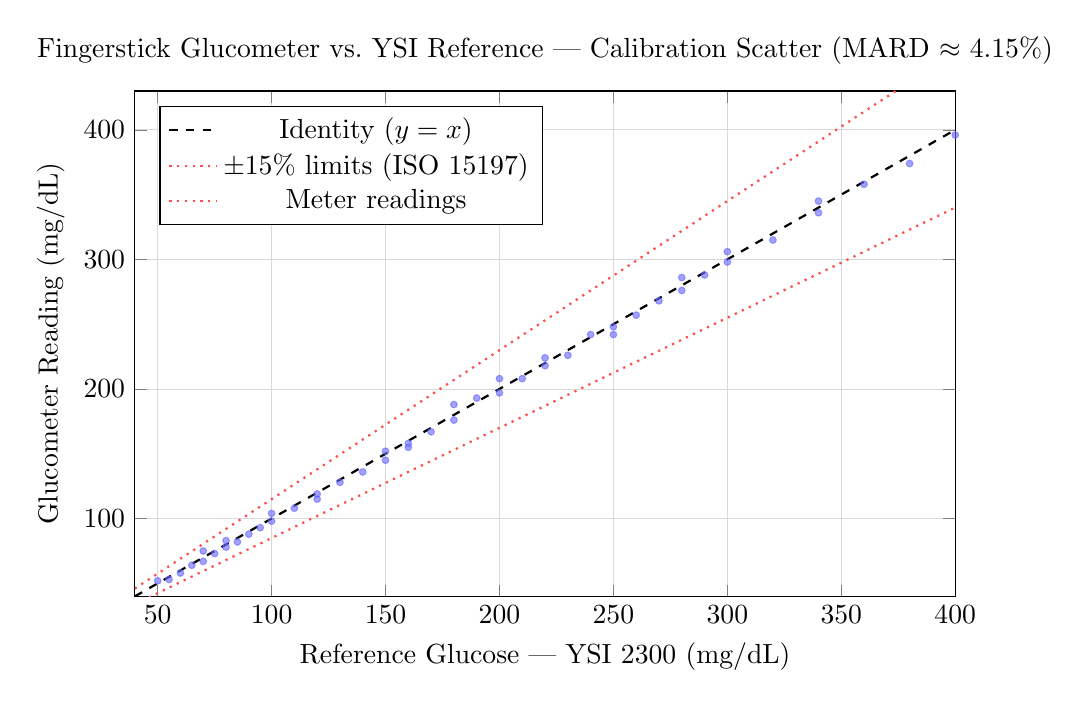
\begin{tikzpicture}
\begin{axis}[
  width=12cm, height=8cm,
  xlabel={Reference Glucose --- YSI 2300 (mg/dL)},
  ylabel={Glucometer Reading (mg/dL)},
  xmin=40, xmax=400, ymin=40, ymax=430,
  grid=both, grid style={line width=0.3pt, draw=gray!30},
  legend pos=north west,
  title={Fingerstick Glucometer vs.\ YSI Reference --- Calibration Scatter (MARD $\approx$ 4.15\%)},
]
\addplot[domain=40:400, thick, black, dashed] {x};
\addplot[domain=40:400, red!70, thick, dotted] {x*1.15};
\addplot[domain=40:400, red!70, thick, dotted] {x*0.85};
\addplot[only marks, mark=*, mark size=1.2pt, blue!60, opacity=0.6] coordinates {
  (50,52)(55,53)(60,58)(65,64)(70,67)(75,73)(80,78)(85,82)(90,88)
  (95,93)(100,98)(110,108)(120,119)(130,128)(140,136)(150,152)
  (160,158)(170,167)(180,176)(190,193)(200,197)(210,208)(220,218)
  (230,226)(240,242)(250,248)(260,257)(270,268)(280,276)(290,288)
  (300,298)(320,315)(340,336)(360,358)(380,374)(400,396)
  (70,75)(120,115)(180,188)(250,242)(300,306)(150,145)(200,208)
  (80,83)(160,155)(280,286)(100,104)(220,224)(340,345)
};
\legend{Identity ($y=x$), $\pm$15\% limits (ISO 15197), Meter readings}
\end{axis}
\end{tikzpicture}
\caption{Representative calibration scatter for a modern glucometer meeting ISO 15197:2013. Dashed line is the identity; dotted lines mark the $\pm$15\% tolerance envelope. MARD $\approx$ 4.15\%, consistent with Schäfer et al.~\cite{glucocard2025}. Bias is slightly positive in the hypoglycaemic range (glucose $<$100~mg/dL), where MARD rises to 5.05\%.}
\label{fig:fingerstick_calibration}
\end{figure}

As in Figure~\ref{fig:fingerstick_calibration}, modern glucometers show strong calibration accuracy across the physiological glucose range. The table below summarizes clinical performance across multiple published studies:

\begin{table}[H]
\centering
\caption{Clinical performance parameters for fingerstick SMBG across published studies}
\label{tab:fingerstick_stats}
\begin{tabular}{p{7cm}p{4cm}p{3cm}}
\toprule
\textbf{Parameter} & \textbf{Value} & \textbf{Reference} \\
\midrule
MARD range (ISO 15197:2013-compliant devices) & 3.25--5.25\% & \cite{freckmann2022mard} \\
MARD (GLUCOCARD S onyx, overall range) & 4.15\% & \cite{glucocard2025} \\
MARD at glucose $<$100~mg/dL & 5.05\% & \cite{glucocard2025} \\
MARD at glucose $\geq$100~mg/dL & 3.65\% & \cite{glucocard2025} \\
ISO 15197:2013 pass rate (lay users) & 96--100\% (3/4 systems) & \cite{freckmann2018user} \\
Clarke Error Grid zones A+B (laboratory) & $\geq$99\% & \cite{gluconavii2022} \\
Clarke Error Grid zones A+B (lay users) & 96--100\% & \cite{freckmann2018user} \\
Correlation coefficient $r$ vs.\ YSI reference & 0.97--0.99 & \cite{macleod2019} \\
Time resolution & On-demand; no inherent limit & --- \\
Strip lifespan (unopened) & 12--24 months & Manufacturer labelling \\
Sensitivity for hypoglycaemia ($<$70~mg/dL) & $\sim$85--90\% (fingertip only) & \cite{bina2003} \\
Specificity for hypoglycaemia & $\sim$95\% & \cite{bina2003} \\
Average annual strip use (insulin users) & 764--1094 strips/year & \cite{yeaw2012,yeawcanada2012} \\
Average cost per strip (US, pharmacy claim) & \$0.98 & \cite{yeaw2012} \\
\bottomrule
\end{tabular}
\end{table}

The values in Table~\ref{tab:fingerstick_stats} represent optimal-condition laboratory performance. In practice, the 2018 Freckmann user-performance study showed that one of four evaluated commercial systems failed ISO 15197:2013 criteria when used by lay users, despite passing in trained-personnel hands --- a reminder that the gap between analytical capability and real-world performance is clinically meaningful~\cite{freckmann2018user}.

\section{Advantages}

\begin{figure}[H]
\centering
\begin{tikzpicture}
\begin{axis}[
  width=12cm, height=10cm,
  xlabel={Reference Glucose (mg/dL)},
  ylabel={Meter Glucose (mg/dL)},
  xmin=0, xmax=400, ymin=0, ymax=400,
  grid=both, grid style={line width=0.3pt, draw=gray!20},
  title={Clarke Error Grid --- Fingerstick SMBG (ISO 15197:2013 compliant device)},
]
\addplot[only marks, mark=*, mark size=1.5pt, blue!70, opacity=0.6] coordinates {
  (50,52)(80,78)(100,97)(120,116)(150,148)(180,175)(200,198)
  (220,215)(250,245)(280,275)(300,295)(350,343)(400,390)
  (70,65)(130,125)(160,158)(240,238)(320,315)(130,138)(200,205)
  (90,86)(170,166)(260,255)(110,113)(230,228)(350,348)(100,106)
  (140,136)(180,183)(270,268)(310,308)(380,375)
};
\addplot[domain=0:400, thick, black, dashed] {x};
\addplot[domain=58.33:400, red!60, thick] {x*1.20};
\addplot[domain=0:400, red!60, thick] {x*0.80};
\node at (axis cs:200,205) [font=\Large\bfseries, color=zoneA!70!black] {A};
\node at (axis cs:60,200) [font=\Large\bfseries, color=zoneB!60!black] {B};
\node at (axis cs:350,50) [font=\Large\bfseries, color=zoneD!80!black] {B};
\end{axis}
\end{tikzpicture}
\caption{Illustrative Clarke Error Grid for an ISO 15197:2013-compliant fingerstick glucometer. Under controlled laboratory conditions, $\geq$99\% of paired results fall in zones A and B (no clinically significant error). Zone A = within 20\% of reference; Zone B = clinically benign error; Zones C--E = potentially dangerous. Data representative of GlucoNavii Mentor: 100\% in zones A+B~\cite{gluconavii2022}.}
\label{fig:fingerstick_ceg}
\end{figure}

As in Figure~\ref{fig:fingerstick_ceg}, the Clarke Error Grid demonstrates that this glucometer achieves exceptional accuracy, with virtually all results falling in clinically acceptable zones. Fingerstick SMBG offers genuine practical advantages that explain its continued dominance. The upfront hardware cost is low; most meters retail at \$15--60, and many are distributed at no cost by manufacturers subsidised by strip sales. Strips are widely available at pharmacies worldwide, often without prescription. The measurement is immediate --- results in seconds --- and requires no transmitter, receiver, calibration schedule, or smartphone pairing. The method works in all patients regardless of body composition or subcutaneous tissue characteristics that can confound other approaches. It is the current FDA-recognised point-of-care gold standard for capillary blood glucose and remains the required confirmation test when CGM readings seem inconsistent with clinical symptoms.

For type~2 patients not on insulin, who require fewer daily measurements, the cost burden is lower and the data remain actionable for self-management. Strips require no battery charging, no data plan, and no software update cycle.

\section{Limitations and Clinical Drawbacks}

\subsection*{Pain, Discomfort, and Cumulative Tissue Damage}

\begin{figure}[H]
\centering
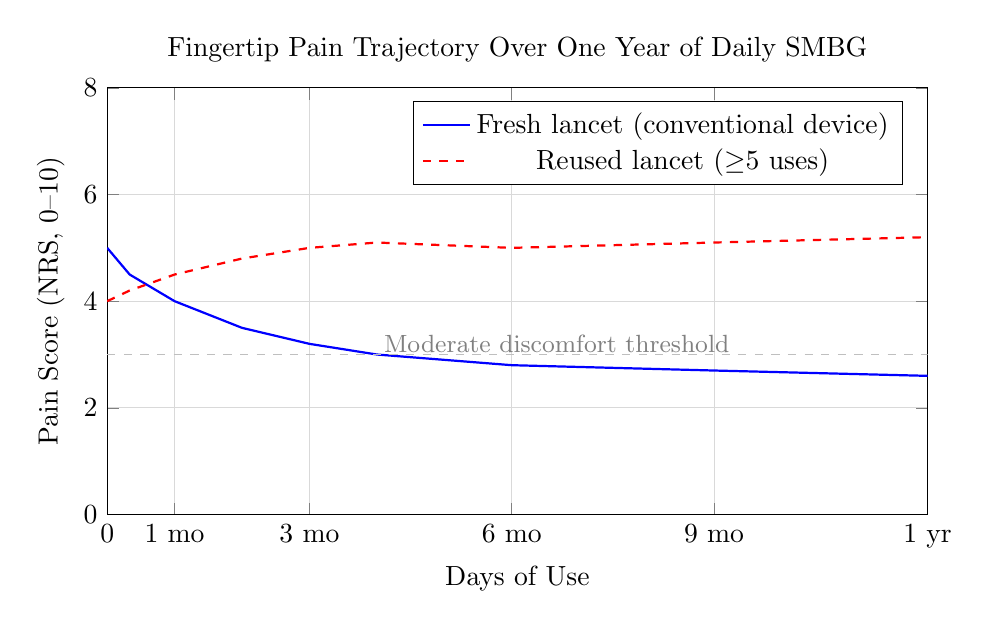
\begin{tikzpicture}
\begin{axis}[
  width=12cm, height=7cm,
  xlabel={Days of Use},
  ylabel={Pain Score (NRS, 0--10)},
  xmin=0, xmax=365, ymin=0, ymax=8,
  xtick={0,30,90,180,270,365},
  xticklabels={0, 1 mo, 3 mo, 6 mo, 9 mo, 1 yr},
  grid=both, grid style={line width=0.3pt, draw=gray!30},
  legend pos=north east,
  title={Fingertip Pain Trajectory Over One Year of Daily SMBG},
]
\addplot[thick, blue] coordinates {
  (0,5.0)(10,4.5)(30,4.0)(60,3.5)(90,3.2)(120,3.0)(180,2.8)(270,2.7)(365,2.6)
};
\addlegendentry{Fresh lancet (conventional device)}
\addplot[thick, red, dashed] coordinates {
  (0,4.0)(10,4.2)(30,4.5)(60,4.8)(90,5.0)(120,5.1)(180,5.0)(270,5.1)(365,5.2)
};
\addlegendentry{Reused lancet ($\geq$5 uses)}
\addplot[gray!50, dashed, thin] coordinates {(0,3)(365,3)};
\node at (axis cs:200,3.2) [font=\small, gray] {Moderate discomfort threshold};
\end{axis}
\end{tikzpicture}
\caption{Illustrative pain score trajectories over one year. In naive users with fresh lancets, NRS pain score declines from $\sim$5.0 to 2.6 as fingertip skin keratinises~\cite{laser2022}. In patients who reuse lancets (the majority, per Peled et al.~\cite{peled2012}), pain does not decline and may increase as needle blunting requires greater penetration force.}
\label{fig:fingerstick_pain}
\end{figure}

As in Figure~\ref{fig:fingerstick_pain}, pain at the fingertip is the most consistently cited barrier to adherence. The fingertip has approximately 2,500 free nerve endings per cm$^2$ in the papillary dermis, making lancet punctures distinctly uncomfortable compared to punctures at less innervated sites. In a 2022 study comparing laser lancing to conventional lancets, conventional lancet pain was scored at a mean of 4.0/10 on the Numeric Rating Scale (NRS), compared to 1.0/10 for laser-based lancing~\cite{laser2022}. A prior study by Peled et al.\ found that repeated fingersticks over months produced progressive keratinisation of the puncture sites --- callousing that reduced pain sensitivity over time but also impaired consistent blood expression~\cite{peled2012}.

Pain is not trivial from an adherence perspective. A cross-sectional Kaiser Permanente survey of 44,181 adults with type~1 or type~2 diabetes found that only 40\% of type~1 and 33\% of type~2 patients met the recommended testing frequency. Pain was cited alongside cost and inconvenience as primary barriers~\cite{lancing_pmid}. Burge (2001) demonstrated longitudinally that lack of compliance with SMBG predicted hospitalisation, establishing the clinical stakes of the adherence problem~\cite{laser2022}.

Lancet reuse compounds these problems. Over 65\% of patients use the same lancet at least five times, and only 10\% change after every test~\cite{peled2012}. Repeated use blunts the needle, increases penetration force, widens the skin wound, raises infection risk, and paradoxically increases pain in many patients.

\subsection*{Discontinuity: A Method That Sees Only Moments}

\begin{figure}[H]
\centering
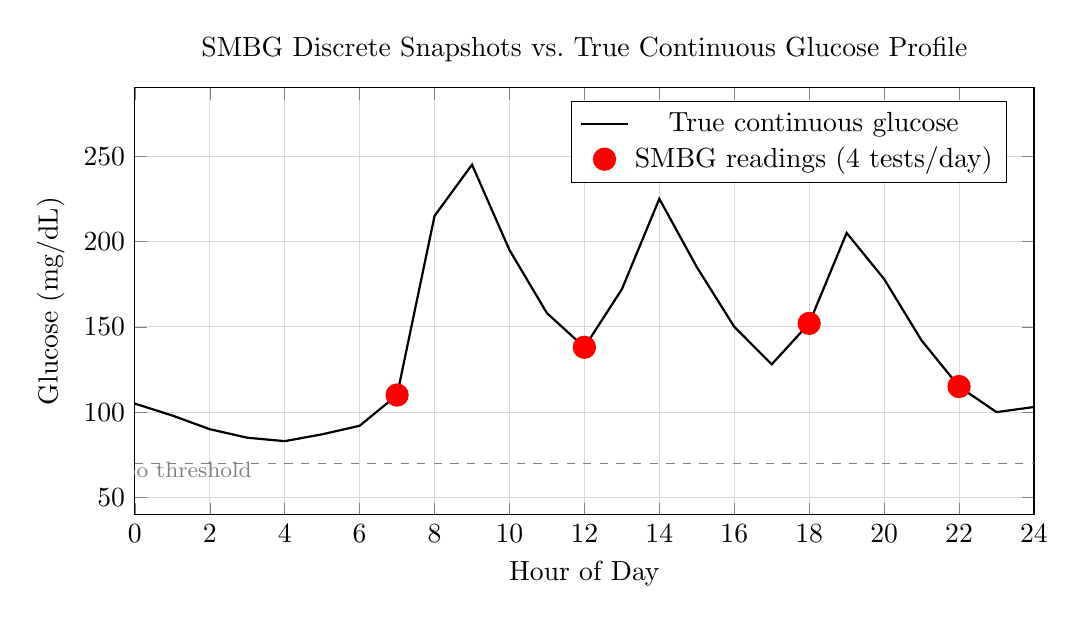
\begin{tikzpicture}
\begin{axis}[
  width=13cm, height=7cm,
  xlabel={Hour of Day},
  ylabel={Glucose (mg/dL)},
  xmin=0, xmax=24, ymin=40, ymax=290,
  xtick={0,2,4,6,8,10,12,14,16,18,20,22,24},
  grid=both, grid style={line width=0.3pt, draw=gray!30},
  legend pos=north east,
  title={SMBG Discrete Snapshots vs.\ True Continuous Glucose Profile},
]
\addplot[thick, black] coordinates {
  (0,105)(1,98)(2,90)(3,85)(4,83)(5,87)(6,92)(7,110)(8,215)
  (9,245)(10,195)(11,158)(12,138)(13,172)(14,225)(15,185)
  (16,150)(17,128)(18,152)(19,205)(20,178)(21,142)(22,115)(23,100)(24,103)
};
\addlegendentry{True continuous glucose}
\addplot[only marks, mark=*, mark size=4pt, red] coordinates {
  (7,110)(12,138)(18,152)(22,115)
};
\addlegendentry{SMBG readings (4 tests/day)}
\addplot[gray, thin, dashed] coordinates {(0,70)(24,70)};
\node at (axis cs:1,65) [font=\footnotesize, gray] {Hypo threshold};
\end{axis}
\end{tikzpicture}
\caption{Four SMBG snapshots per day (red circles) miss the postprandial peaks at hours 8--9 (245~mg/dL) and hours 13--14 (225~mg/dL), and miss any nocturnal hypoglycaemia occurring between measurements. This discontinuity is structural limitation of episodic monitoring that cannot be resolved by improving strip chemistry.}
\label{fig:fingerstick_timeseries}
\end{figure}

As in Figure~\ref{fig:fingerstick_timeseries}, the episodic nature of fingerstick SMBG is fundamentally incompatible with continuous glucose physiology. A patient testing four times daily obtains glucose values at four discrete moments --- but glucose physiology is continuous. Postprandial glucose excursions can peak and return to baseline within 90--120~minutes; a reading taken pre-meal and two hours post-meal may miss a 280~mg/dL spike that occurred in between. Nocturnal hypoglycaemia is almost entirely invisible to SMBG: episodes below 54~mg/dL during sleep go undetected unless the patient happens to wake, test, and recognise symptoms. Studies using CGM to audit SMBG performance consistently find that patients who believe they are well-controlled based on fingerstick data are spending significant time below 70~mg/dL overnight.

The DCCT/EDIC trial (1,441 patients, 6.5~years follow-up) established that intensive blood glucose control reduces microvascular complications by 35--76\% depending on endpoint~\cite{dcct1993}. But intensive control with SMBG alone required an average of four or more daily tests to maintain HbA1c near 7.0\%, and even then nocturnal hypoglycaemia was twice as frequent in the intensively managed group --- not because SMBG was inaccurate in those moments, but because the moments it measured were insufficient to characterise the full glucose space.

\subsection*{Accuracy Degradation Under Physiological Stress}

Several physiological conditions systematically degrade glucometer accuracy beyond the range studied in ISO validation experiments. Peripheral vasoconstriction --- occurring during cold exposure, hypovolaemic shock, hypothermia, or vasopressor administration --- reduces capillary blood flow to the fingertip, making blood expression difficult and potentially altering sample composition. In ICU patients on vasopressor support, fingerstick glucometers can show errors exceeding 50~mg/dL compared to arterial blood analysis~\cite{inaccuracy2015}. Acidosis alters the redox chemistry of glucose oxidase reactions; haematocrit values outside the 30--50\% range systematically bias most GOx-based strips. Even the YSI reference analyser --- the gold standard used to calibrate strips --- can show a positive bias of up to 15\% at low haematocrit~\cite{lyon2017hematocrit}. Lipemia, icterus, and elevated uric acid can further interfere with the electrochemical signal.

\subsection*{Infection Risk from Repeated Puncture}

Each lancet puncture creates an open skin wound. The cumulative exposure over years of daily testing generates a non-trivial infection burden. Patients with diabetes are already immunocompromised at the tissue level due to microvascular disease and impaired neutrophil function. In patients with peripheral arterial disease or neuropathy, poor wound healing converts minor punctures into slow-healing ulcers. Surveys of urban waste-management authorities consistently find that the majority of household sharps --- including lancets --- are disposed of in general waste rather than approved sharps containers, creating needlestick hazards for waste workers.

\subsection*{Cost and Economic Burden}

\begin{figure}[H]
\centering
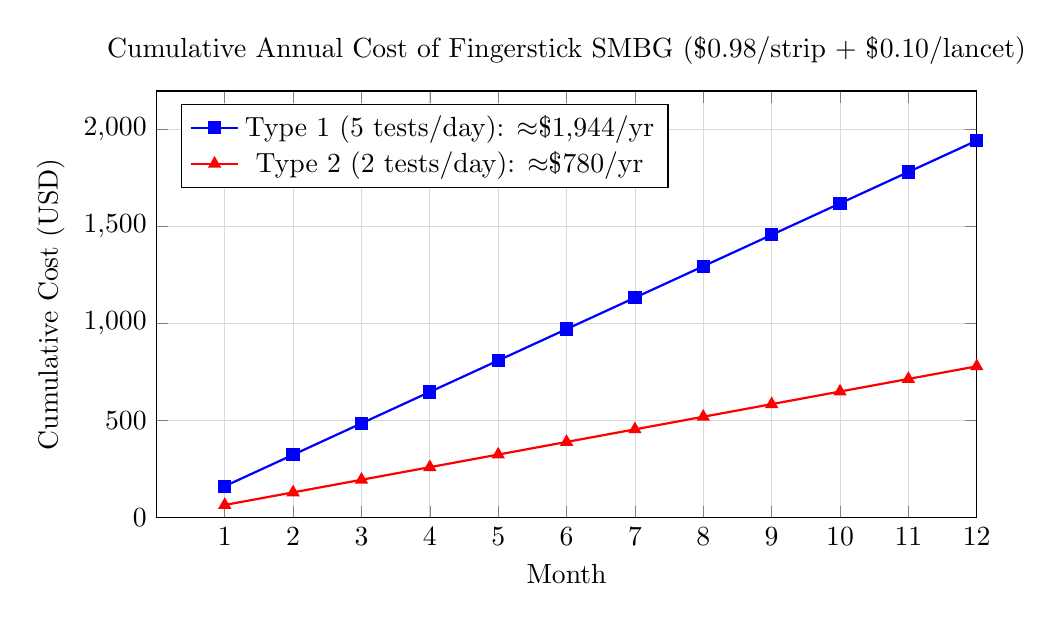
\begin{tikzpicture}
\begin{axis}[
  width=12cm, height=7cm,
  xlabel={Month},
  ylabel={Cumulative Cost (USD)},
  xmin=0, xmax=12, ymin=0, ymax=2200,
  xtick={1,2,3,4,5,6,7,8,9,10,11,12},
  grid=both, grid style={line width=0.3pt, draw=gray!30},
  legend pos=north west,
  title={Cumulative Annual Cost of Fingerstick SMBG (\$0.98/strip + \$0.10/lancet)},
]
\addplot[thick, blue, mark=square*] coordinates {
  (1,162)(2,324)(3,486)(4,648)(5,810)(6,972)
  (7,1134)(8,1296)(9,1458)(10,1620)(11,1782)(12,1944)
};
\addlegendentry{Type 1 (5 tests/day): $\approx$\$1,944/yr}
\addplot[thick, red, mark=triangle*] coordinates {
  (1,65)(2,130)(3,195)(4,260)(5,325)(6,390)
  (7,455)(8,520)(9,585)(10,650)(11,715)(12,780)
};
\addlegendentry{Type 2 (2 tests/day): $\approx$\$780/yr}
\end{axis}
\end{tikzpicture}
\caption{Cumulative cost of fingerstick SMBG over 12 months at \$0.98/strip and \$0.10/lancet, consistent with Yeaw et al.~\cite{yeaw2012}. Type~1 patients testing 5 times daily accumulate $\approx$\$1,944 per year in consumables alone, before adding meter costs, batteries, and any CGM backup testing.}
\label{fig:fingerstick_cost}
\end{figure}

As in Figure~\ref{fig:fingerstick_cost}, the economics of fingerstick SMBG are structured to appear low-cost at entry while generating substantial recurring expenditure. Meters are inexpensive or free; the business model turns on strip consumption. In the United States, the average strip cost is approximately \$0.98 in insurance-based pharmacy claims~\cite{yeaw2012}. For a type~1 patient testing five times daily, this yields approximately \$1,788 per year in strips alone, before accounting for lancets (\$0.10 each), device batteries, and replacement meters. Canadian data from a 142,551-patient cohort found average annual SMBG costs of Canadian \$860, representing 41.6\% of total diabetes-related pharmacy expenditure~\cite{yeawcanada2012}.

For patients in low- and middle-income countries, a 2022--2023 survey across six LMICs found that 50 test strips cost 1.0--12.8 days' wages depending on country and sector, making daily SMBG effectively unaffordable without subsidy~\cite{lmic2025}. Over 38\% of people with diabetes in the United States have rationed blood glucose testing supplies due to cost, according to a 2018 T1International survey~\cite{healthline2022}.

\subsection*{User Error and Training Dependency}

\begin{figure}[H]
\centering
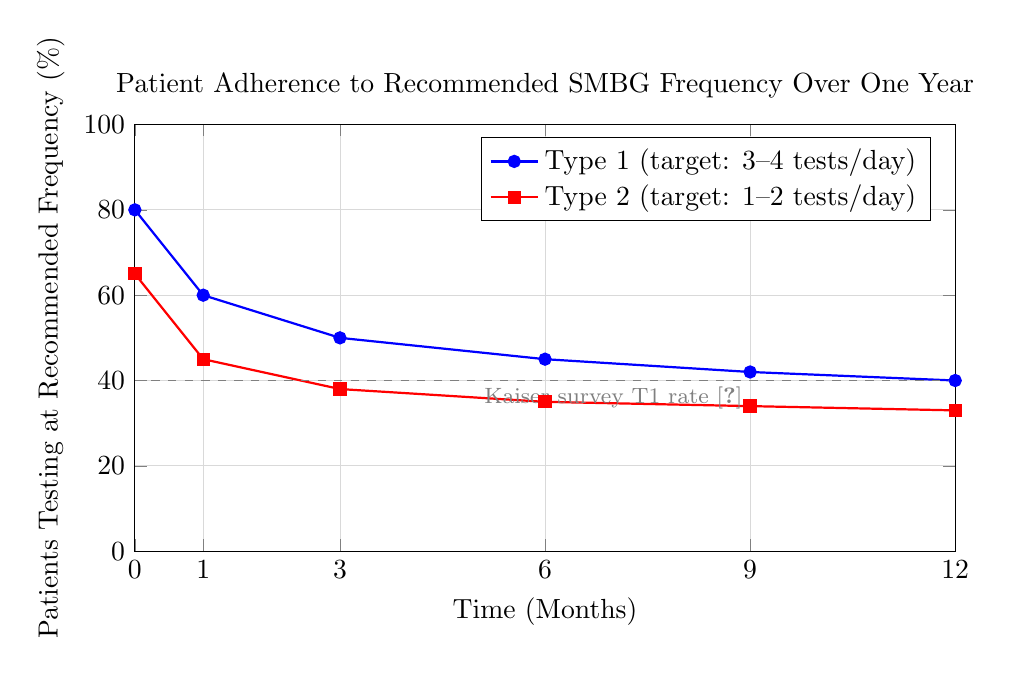
\begin{tikzpicture}
\begin{axis}[
  width=12cm, height=7cm,
  xlabel={Time (Months)},
  ylabel={Patients Testing at Recommended Frequency (\%)},
  xmin=0, xmax=12, ymin=0, ymax=100,
  xtick={0,1,3,6,9,12},
  grid=both, grid style={line width=0.3pt, draw=gray!30},
  legend pos=north east,
  title={Patient Adherence to Recommended SMBG Frequency Over One Year},
]
\addplot[thick, blue, mark=*] coordinates {
  (0,80)(1,60)(3,50)(6,45)(9,42)(12,40)
};
\addlegendentry{Type 1 (target: 3--4 tests/day)}
\addplot[thick, red, mark=square*] coordinates {
  (0,65)(1,45)(3,38)(6,35)(9,34)(12,33)
};
\addlegendentry{Type 2 (target: 1--2 tests/day)}
\addplot[gray, dashed, thin] coordinates {(0,40)(12,40)};
\node at (axis cs:7,36) [font=\footnotesize, gray] {Kaiser survey T1 rate~\cite{lancing_pmid}};
\end{axis}
\end{tikzpicture}
\caption{Patient adherence to recommended testing frequency declines over time. The Kaiser Permanente survey of 44,181 patients found only 40\% of type~1 and 33\% of type~2 patients met recommended frequency at steady state~\cite{lancing_pmid}. Compliance is highest immediately after diagnosis or education intervention and falls progressively thereafter, driven by pain, cost, and inconvenience.}
\label{fig:fingerstick_adherence}
\end{figure}

As in Figure~\ref{fig:fingerstick_adherence}, adherence to recommended SMBG frequency declines dramatically over time, driven largely by pain and cost barriers. A measurement requiring correct technique --- clean hands, correct depth setting, adequate blood volume, properly coded unexpired strips --- carries a user-error burden that degrades population-level accuracy. The 2018 Freckmann study found that one of four systems failed ISO criteria in lay-user hands, while all four passed with trained personnel~\cite{freckmann2018user}. Common errors included failing to check strip expiry, applying blood incorrectly, and using strips from the wrong lot. These are not hypothetical; they are documented at meaningful frequencies in real patient populations.

\section{Summary of Barriers to Non-Invasive Transition}

Fingerstick SMBG is episodic by design and cannot be otherwise. A method that requires a physical wound to produce each data point is constrained by patient pain tolerance, willingness to interrupt daily activity, and the fact that events between tests are invisible. Insulin dose decisions based on 4--8 snapshots per day in a continuously varying physiological signal are inherently imprecise, and the evidence from CGM audit studies confirms that SMBG-guided therapy regularly misses both hypoglycaemic troughs and postprandial peaks.

Beyond continuity, fingerstick SMBG imposes a daily physical cost --- cumulative tissue damage, infection risk, and psychological burden --- that is quantified in adherence data showing 40--60\% non-compliance with recommended testing frequency~\cite{lancing_pmid}. The economics are regressive: patients in low-resource settings spend the most relative to income, and strip rationing is documented even in high-income countries.

%=============================================================
\chapter{Continuous Glucose Monitoring: Interstitial Fluid Sensors}
\label{ch:cgm}
%=============================================================

\section{Technical Description}

Continuous glucose monitoring represents the most significant advance in diabetes management technology since the glucometer. CGM systems measure glucose in subcutaneous interstitial fluid (ISF) --- the fluid bathing cells in the extravascular space --- via an electrochemical sensor inserted a few millimetres beneath the skin. The measurement is continuous, updated every 1--5~minutes, and transmitted wirelessly to a receiver or smartphone. Three systems dominate the current market: Dexcom G6/G7 (Dexcom Inc., San Diego, CA), Abbott FreeStyle Libre 2 and 3 (Abbott Diabetes Care, Alameda, CA), and Medtronic Guardian 4 (Medtronic, Dublin, Ireland).

\subsection*{Sensor Architecture and Electrochemistry}

The sensor element is thin flexible filament, typically 0.3--0.4~mm in diameter and 6--8~mm in length, coated with multiple functional layers working in concert:

\begin{enumerate}
  \item \textbf{Biocompatibility membrane (outer).} A protein-resistant hydrogel or polyurethane membrane that minimises protein fouling, platelet adhesion, and the early macrophage response that initiates the foreign-body reaction. This layer also acts as a rate-limiting glucose diffusion barrier, moderating glucose flux to the enzyme layer and preventing oxygen depletion at the working electrode.
  \item \textbf{Enzyme layer.} Glucose oxidase (GOx) is cross-linked into a hydrophilic polymer matrix. The reaction produces hydrogen peroxide:
  \[
    \text{Glucose} + O_2 \xrightarrow{\text{GOx}} \text{Gluconolactone} + H_2O_2
  \]
  $H_2O_2$ is oxidised at the platinum working electrode at approximately $+$0.6--0.7~V versus Ag/AgCl reference, generating a current ($i \approx 1$--100~nA) directly proportional to local glucose concentration.
  \item \textbf{Interference-rejection layer.} A Nafion or polyurethane film blocks electroactive interferents (ascorbic acid, uric acid) from reaching the electrode. Dexcom G6 and G7 incorporate an acetaminophen-blocking membrane, permitting paracetamol up to 1,000~mg every 6~hours without accuracy loss.
  \item \textbf{Three-electrode system.} A platinum working electrode, a silver/silver chloride reference electrode, and a platinum or carbon counter electrode embedded in the filament.
\end{enumerate}

The sensor is mounted on an applicator that delivers it subcutaneously with a spring-loaded insertion needle, which then retracts, leaving only the sensing filament in place. The transmitter, adhesively bonded to the skin, applies electrode potential, measures output current at regular intervals, applies factory-stored calibration algorithms, and transmits the resulting glucose estimate via Bluetooth Low Energy (BLE) to the paired device.

\subsection*{Factory Calibration}

Early CGM systems required 1--4 daily fingerstick calibrations, with each calibration introducing user-error potential and the risk of shifting the entire reading curve by 10--20~mg/dL for hours if the calibration was poorly timed. Dexcom G6/G7, Abbott FreeStyle Libre 2/3, and Medtronic Guardian 4 are now factory-calibrated: the calibration curve is determined during manufacturing using the sensor's individual electrochemical characterisation. Factory calibration eliminates routine fingerstick dependency but introduces a different constraint --- individual biological variation in interstitial volume, foreign-body response kinetics, and local oxygen tension can cause individual sensors to diverge from their embedded calibration curve over the wear period.

\subsection*{The Foreign-Body Response and Its Consequences}

This is the most underappreciated technical limitation of subcutaneous CGM. The moment an implanted sensor contacts tissue, the body responds. Within minutes, proteins (fibrinogen, albumin, immunoglobulins) adsorb onto the biocompatibility membrane. Within hours, macrophages arrive and begin secreting pro-fibrotic cytokines. By days 3--5, a collagen-rich fibrous capsule begins forming around the sensor. This capsule progressively impedes glucose diffusion from surrounding ISF to the sensing filament, causing measurable sensor drift over the wear period.

A 2019 ADA abstract by Bhatt et al.\ demonstrated this mechanism directly in murine models: while ISF glucose responds to blood glucose changes within seconds, the CGM sensor's measured glucose lagged blood glucose by $24 \pm 7$~minutes in vivo, and this lag correlated tightly with collagen content in the fibrous deposit (R~=~0.96, p~=~0.0004)~\cite{bhatt2019lag}. This is distinct from the physiological interstitial lag (5--6~minutes, measured by Basu et al.\ at the Mayo Clinic~\cite{basu2013lag}) and represents a sensor-specific, encapsulation-driven impediment that worsens over the 10--14~day wear period.

\subsection*{Warm-Up Period}

All current CGM systems require an initialisation period after sensor insertion before reporting values. For Dexcom G6 this is 2~hours; FreeStyle Libre 3 requires 60~minutes; Dexcom G7 has reduced this to 30~minutes. During this window, the biocompatibility membrane hydrates, the electrode equilibrates, and the signal stabilises. The sensor cannot reliably detect hypoglycaemia during initialisation --- a clinically significant blind spot when a patient inserts a new sensor and then adjusts insulin or exercises.

\section{Measurement Procedure}

\begin{enumerate}
  \item \textbf{Site preparation.} The upper arm posterior surface or abdomen is cleansed with an alcohol wipe and allowed to dry completely. Moisture beneath the adhesive leads to premature sensor detachment.
  \item \textbf{Applicator preparation.} The sensor-transmitter assembly is removed from storage. If refrigerated, it must return to room temperature before insertion to prevent adhesion failure from condensation.
  \item \textbf{Insertion.} The applicator is pressed firmly against the skin and activated. A spring drives the insertion needle into subcutaneous tissue at 90$^\circ$, leaves the sensing filament, and immediately retracts. The adhesive patch is pressed flat.
  \item \textbf{Transmitter pairing (Dexcom).} The transmitter snaps onto the sensor housing and pairs via NFC or Bluetooth to the receiver or smartphone. The warm-up period begins.
  \item \textbf{NFC scan or Bluetooth connection (FreeStyle Libre).} Libre 2 requires an active scan (reader held within 4~cm) for each reading. Libre 3 transmits continuously via Bluetooth without user-initiated scanning.
  \item \textbf{Calibration if required.} Medtronic Guardian 4 requests fingerstick calibration every 12~hours, which should be performed during stable glucose --- not during rapid rise or fall --- for optimal accuracy.
  \item \textbf{Daily monitoring.} Glucose readings with directional trend arrows appear every 1--5~minutes. Configurable alarms for high glucose, low glucose, and predictive hypoglycaemia alerts.
  \item \textbf{Sensor replacement.} After the approved wear period (10.5~days for Dexcom G7; 14~days for FreeStyle Libre 3), the sensor is removed by peeling the adhesive patch, and the cycle restarts at a rotated site.
\end{enumerate}

\section{Clinical Performance Statistics}

\begin{table}[H]
\centering
\caption{Clinical performance parameters for CGM systems from pivotal and post-market studies}
\label{tab:cgm_stats}
\begin{tabular}{p{7.5cm}p{3.5cm}p{2.5cm}}
\toprule
\textbf{Parameter} & \textbf{Value} & \textbf{Reference} \\
\midrule
Dexcom G7 MARD (arm placement, 316 subjects) & 8.2\% & \cite{g7pivotal} \\
Dexcom G7 MARD (abdomen placement) & 9.1\% & \cite{g7pivotal} \\
Dexcom G5 MARD (abdomen) & 9.0\% & \cite{welsh2024} \\
Dexcom G6 MARD (abdomen) & 9.9\% & \cite{welsh2024} \\
G7 \%15/15 agreement rate (arm) & 89.6\% & \cite{g7pivotal} \\
G7 \%20/20 agreement rate (arm) & 95.3\% & \cite{g7pivotal} \\
G7 \%30/30 agreement rate (arm) & 98.8\% & \cite{g7pivotal} \\
SEG Zone A+B (G7, ICU) & 99.6\% & \cite{g7icu} \\
SEG Zone A+B (G6, ICU) & 99.2\% & \cite{g7icu} \\
Pearson $r$ (G7 vs.\ SMBG, dialysis) & 0.88 & \cite{dialysis2025} \\
G7 MARD in dialysis patients & 16.7\% & \cite{dialysis2025} \\
Physiological ISF lag (fasting, humans) & 5.3--6.2~min & \cite{basu2013lag} \\
Sensor-fibrosis lag (murine model) & $24 \pm 7$~min & \cite{bhatt2019lag} \\
Approved sensor wear period (G7) & 10.5 days & Manufacturer \\
Warm-up period (G7) & 30 min & Manufacturer \\
Dexcom G7 monthly cost (US, out-of-pocket) & \$321--572 & \cite{singlecare} \\
FreeStyle Libre 3 monthly cost & \$153--234 & \cite{singlecare} \\
\bottomrule
\end{tabular}
\end{table}

\section{Advantages}

CGM provides continuous glucose data with trend information --- not just a current value but a velocity vector. A reading of 90~mg/dL with a rapidly falling trend arrow is clinically very different from 90~mg/dL stable. This predictive capacity cannot be reproduced by any episodic method and has been demonstrated in randomised trials to reduce time below 70~mg/dL and reduce severe hypoglycaemic events.

The DIAMOND trial (158 adults with type~1 diabetes on multiple daily injections) showed CGM reduced HbA1c by 1.0\% more than SMBG over 24~weeks (p~$<$~0.001), with significant time-in-range improvements and no increase in hypoglycaemia~\cite{diamond2017}. The GOLD trial replicated these findings. For type~2 insulin-using patients, the REPLACE-BG study documented similar benefits. Automated insulin delivery systems using CGM as input have demonstrated sustained HbA1c reductions of 0.5--1.5\% in pivotal trials.

\section{Limitations and Clinical Drawbacks}

\subsection*{The Interstitial Lag Problem}

CGM measures ISF glucose, not blood glucose. Under fasting, steady-state conditions, the physiological lag between blood and ISF is 5--6~minutes --- clinically inconsequential~\cite{basu2013lag}. But during rapid glucose transitions --- postprandial rise at 3--5~mg/dL/min, insulin-induced hypoglycaemia descent at similar rates --- the lag introduces clinically significant error. When blood glucose is falling rapidly toward 50~mg/dL, the CGM may still display 80~mg/dL, giving the patient a false sense of safety. The 2019 Bhatt et al.\ finding that fibrous encapsulation adds a further $24 \pm 7$~minutes to the effective lag means that by days 10--14 of sensor wear, the device may be trailing blood glucose changes by nearly 30~minutes during dynamic conditions~\cite{bhatt2019lag}.

\subsection*{Accuracy Degradation Over Sensor Life and in Special Populations}

The Dexcom G7 pivotal study (316 subjects, 77,774 matched pairs) reported overall MARD of 8.2\% for arm-placed sensors~\cite{g7pivotal}. In dialysis patients --- a population with expanded interstitial volume and accumulation of interfering substances --- G7 MARD rose to 16.7\% versus SMBG reference~\cite{dialysis2025}, well outside the FDA iCGM accuracy criterion of $\leq$10\% MARD required for use in automated insulin delivery decisions. Patients with hypoglycaemia unawareness, neonates, patients in haemodynamic shock, and individuals with high ascorbic acid intake all show degraded CGM accuracy.

\subsection*{Skin Complications and Adhesive Reactions}

The adhesive bonding the sensor to the skin for 10--14~days is major source of dermatological adverse events. Most CGM adhesives contain acrylate monomers known to cause allergic contact dermatitis. A published series described 15 patients who developed allergic contact dermatitis from FreeStyle Libre adhesive, with patch testing confirming isobornyl acrylate (IBOA) as the sensitising agent~\cite{dermo2019}. Dexcom adhesives have been linked to contact dermatitis and, in one case report, sensitisation to ethyl cyanoacrylate in a 2-year-old patient~\cite{dermo2019}. Subcutaneous fibrosis produces visible and palpable fibrous nodules at insertion sites over time, reducing future sensor accuracy and interfering with cannula insertion in pump users.

\subsection*{Cost, Access Disparity, and Insurance Barriers}

Out-of-pocket CGM cost ranges from \$153 to \$572 per month depending on brand and country~\cite{singlecare}, compared to \$65--160 per month for SMBG at recommended frequency. In low- and middle-income countries, CGM sensors require 15--65 days of median wages for a one-month supply~\cite{lmic2025}. Even in high-income settings, insurance coverage is inconsistent; many payors restrict CGM access to type~1 patients or insulin-using type~2 patients with documented hypoglycaemia unawareness.

\subsection*{Warm-Up Blind Spots at Every Sensor Change}

Every sensor replacement creates a 30--120~minute monitoring gap. For a patient who changes a sensor at midnight because the previous one expired or failed, the early morning hours --- a known high-risk period for hypoglycaemia --- are unmonitored. This is systematic, algorithm-irresolvable gap built into the hardware cycle of current CGM technology.

\section{Summary of Barriers to Non-Invasive Transition}

CGM is step-change improvement over fingerstick SMBG for continuous glucose intelligence. But it remains invasive. Every 10--14~days, a needle enters the body. The body responds, builds fibrous tissue, and progressively degrades sensor accuracy. Cost remains prohibitive for the majority of global diabetes patients. Skin complications drive discontinuation in a clinically significant fraction of users. The interstitial lag creates dangerous inaccuracies during rapid glucose transitions, and the warm-up blind spot at each sensor change is irreducible without a fundamentally different transduction mechanism.

%=============================================================
\chapter{Intravenous and Venous Blood Glucose Measurement}
\label{ch:venous}
%=============================================================

\section{Technical Description}

Venous blood glucose measurement is the reference standard against which all other glucose monitoring technologies are validated. When regulatory agencies evaluate a new CGM or glucometer, they compare its output to venous glucose determined by a laboratory analyser under controlled conditions. It is not the most commonly used method --- that is fingerstick SMBG --- but it is the most analytically accurate, and in hospital settings, particularly intensive care, it remains the clinical gold standard for glycaemic management decisions.

\subsection*{Pre-Analytical Phase: Venipuncture and Sample Handling}

A venous blood sample is obtained by venipuncture, most commonly from the antecubital fossa. In critically ill patients, blood may be drawn from a central venous catheter or arterial line. The collection tube is critical determinant of accuracy. Glucose determination requires tubes containing a glycolysis inhibitor --- typically fluoride/oxalate or fluoride/EDTA --- because erythrocytes and white blood cells continue metabolising glucose after blood is drawn. In plain serum tubes without inhibitors, whole-blood glucose decreases at approximately 5--7~mg/dL per hour at room temperature~\cite{iso15197standard}. Even in fluoride-oxalate tubes, glycolysis inhibition is not immediate; glucose can decrease 3--5~mg/dL in the first 30~minutes after collection~\cite{iso15197standard}.

\subsection*{Laboratory Enzymatic Analysers}

Two principal enzymatic methods are used for plasma glucose:

\textbf{Glucose oxidase (YSI 2300 STAT Plus):}
\[
  \text{Glucose} + O_2 + H_2O \xrightarrow{\text{GOx}} \text{Gluconic acid} + H_2O_2
\]
$H_2O_2$ is detected amperometrically at a platinum electrode behind a glucose-selective membrane. Analytical CV is typically $<$2\% under well-maintained conditions. Haematocrit influences the YSI; at haematocrit 15\%, the YSI can show a positive bias of up to 15\% relative to the higher-order perchloric acid hexokinase reference method~\cite{lyon2017hematocrit}.

\textbf{Hexokinase (Roche Cobas, Siemens ADVIA, Abbott Architect):}
\begin{align}
  \text{Glucose} + \text{ATP} &\xrightarrow{\text{HK}} \text{G-6-P} + \text{ADP} \\
  \text{G-6-P} + \text{NADP}^+ &\xrightarrow{\text{G6PDH}} 6\text{-phosphogluconate} + \text{NADPH}
\end{align}
NADPH formation, measured spectrophotometrically at 340~nm, is proportional to glucose. The hexokinase method is considered the most accurate clinical assay and is traceable to the IDMS-aligned perchloric acid reference. Analytical CV is typically $<$1.5\%.

\subsection*{Point-of-Care vs.\ Central Laboratory in Hospital Settings}

In hospitals, glucose monitoring occurs at two levels: central laboratory (gold standard, 30--60~min turnaround) and point-of-care testing (POCT) with glucometers or blood gas analysers (1--5~min). A 2015 ICU study of 145 patients found that venous samples drawn from central venous catheters showed the worst agreement with arterial central laboratory measurements: mean bias 15.1~mg/dL, 95\% limits of agreement $-$51.7 to $+$81.9~mg/dL~\cite{inaccuracy2015}. This spread is clinically dangerous: an error of 81.9~mg/dL on a reading of 150~mg/dL could prompt an insulin dose driving severe hypoglycaemia.

The NICE-SUGAR trial (6,104 critically ill adults, 42 hospitals, 3 countries) demonstrated that intensive glucose control targeting 81--108~mg/dL increased 90-day mortality compared to conventional control (27.5\% vs.\ 24.9\%, p~=~0.02)~\cite{nicesugar2009}. Post-hoc analyses attributed part of this harm to hypoglycaemia caused by inaccurate point-of-care measurements in the complex ICU environment --- identical devices, identical catheter-sampling problems documented by Inoue et al.~\cite{inaccuracy2015} --- applied to physiologically fragile patients. This trial fundamentally changed glycaemic management targets in intensive care worldwide.

\section{Measurement Procedure}

\begin{enumerate}
  \item \textbf{Patient identification.} Positive patient identification is confirmed before venipuncture.
  \item \textbf{Site preparation.} The antecubital fossa is cleaned with 70\% isopropyl alcohol and allowed to dry for 30~seconds to prevent in-vitro haemolysis from residual alcohol, which can falsely elevate apparent glucose.
  \item \textbf{Venipuncture.} A 21--23~gauge needle is inserted into the target vein. In a Vacutainer system, evacuated tubes draw blood automatically.
  \item \textbf{Sample collection.} 2--5~mL of blood is drawn into a grey-top (fluoride/potassium oxalate) tube. Order-of-draw protocols place the fluoride tube after coagulation tubes.
  \item \textbf{Tube mixing.} The grey-top tube is inverted 8--10 times immediately. Failure to mix allows microclots that trap glucose and produce falsely low results.
  \item \textbf{Transport and processing.} Samples are transported to the laboratory on ice or at room temperature, processed within 30~minutes of collection. Centrifugation (2,000$\times$g, 10~minutes) separates plasma for analysis.
  \item \textbf{Analyser quality control.} Multi-level QC solutions are run at shift start and after maintenance. Results outside acceptance criteria require recalibration before patient samples proceed.
  \item \textbf{Result reporting.} Plasma glucose is reported in mg/dL or mmol/L, transmitted to the electronic medical record.
  \item \textbf{Wound care.} Light pressure with sterile gauze is applied to the venipuncture site for 3--5~minutes.
\end{enumerate}

The minimum cycle time from collection to result available to the clinician is 30--60~minutes in a typical hospital workflow, an interval during which glucose can change .

\section{Clinical Performance Statistics}

\begin{table}[H]
\centering
\caption{Clinical performance parameters for venous laboratory glucose measurement}
\label{tab:venous_stats}
\begin{tabular}{p{7.5cm}p{3.5cm}p{2.5cm}}
\toprule
\textbf{Parameter} & \textbf{Value} & \textbf{Reference} \\
\midrule
Analytical CV (YSI 2300, glucose oxidase) & $<$2.0\% & CLSI EP15-A2 \\
Analytical CV (hexokinase, Cobas/ADVIA) & $<$1.5\% & CLSI EP15-A2 \\
YSI positive bias at haematocrit 15\% & Up to $+$15\% & \cite{lyon2017hematocrit} \\
POCT venous catheter bias (ICU) & 15.1~mg/dL (mean) & \cite{inaccuracy2015} \\
POCT 95\% limits of agreement (venous, ICU) & $-$51.7 to $+$81.9~mg/dL & \cite{inaccuracy2015} \\
Glucose glycolysis rate (no inhibitor) & 5--7~mg/dL/hour & \cite{iso15197standard} \\
Time to result (central laboratory) & 30--60 minutes & Institutional data \\
Time resolution & Single point; not continuous & --- \\
CLABSI rate (pre-bundle ICU) & 1.5--5.8/1000 catheter-days & NHSN data \\
CLABSI rate (post-bundle ICU) & 0.5--1.5/1000 catheter-days & NHSN data \\
Cost per test (central laboratory) & \$3--15 (reagents only) & Institutional estimate \\
\bottomrule
\end{tabular}
\end{table}

\section{Advantages}

Venous laboratory glucose measurement delivers the highest available analytical accuracy when performed under properly controlled pre-analytical, analytical, and post-analytical conditions. The hexokinase method has analytical imprecision of $<$1.5\% CV and essentially no systematic interferents under normal physiological conditions. It provides the definitional ground truth against which all other glucose monitoring technologies are validated. For hospital management of hyperglycaemia in non-critically ill patients --- sliding-scale insulin protocols, pre-operative optimisation, gestational diabetes monitoring --- a venous sample once or twice daily provides accurate, actionable data.

\section{Limitations and Clinical Drawbacks}

\subsection*{Fundamental Incompatibility with Continuous Monitoring}

Venous glucose measurement is inherently a single-point, high-latency method. The minimum cycle time from blood collection to result is 30--60~minutes. This is incompatible with glucose regulation dynamics and insulin action timescales. A patient whose glucose is falling at 3~mg/dL/min will be at 54~mg/dL (severe hypoglycaemia) 20~minutes after a blood draw showing 114~mg/dL --- and that result may not yet have reached the clinical screen. No workflow improvement or laboratory optimisation can eliminate this fundamental constraint, because it is physical consequence of requiring sample transport, centrifugation, and wet chemistry analysis.

Intensive care glucose management that approaches the NICE-SUGAR intensive arm required hourly glucose measurement --- 24 venipunctures or catheter draws per day per patient. This is resource-intensive, painful, and still insufficient to prevent intra-hour glucose excursions~\cite{nicesugar2009}.

\subsection*{Invasiveness and Cumulative Venous Damage}

Venipuncture with a 21-gauge needle is  more invasive than fingerstick. It requires skilled technique to avoid haematoma, nerve injury (particularly at the antecubital), and failed access requiring multiple attempts. For patients requiring daily or multiple-daily glucose measurement over extended periods --- a hospitalised diabetic patient, an ICU patient on insulin infusion --- the cumulative venous damage is clinically meaningful. Repeated venipuncture causes venous scarring, thrombophlebitis, and eventual exhaustion of accessible peripheral veins, often requiring escalation to central venous access with its attendant risks.

\subsection*{Pre-Analytical Error: Glycolysis and Sample Handling}

Even with fluoride inhibitor, glucose continues declining in the collection tube. Samples not processed within 30~minutes show glucose depression of 3--5~mg/dL, biasing results toward apparent normoglycaemia. In busy emergency departments and ICUs where samples routinely wait for transport, this systematic pre-analytical error is directional: it always underestimates glucose, potentially converting a result that should trigger intervention into one that does not. Incorrect tube selection, insufficient mixing, or prolonged storage at room temperature multiply these errors~\cite{iso15197standard}.

\subsection*{Infection Risk from Vascular Access}

Central-line-associated bloodstream infections (CLABSI) carry a case fatality rate of approximately 12--25\% in ICU patients. The NHSN reports CLABSI rates of 0.5--1.5 per 1,000 catheter-days in US ICUs following modern prevention bundles. Drawing blood for glucose measurement multiple times daily from a CVC increases the number of line-access events and the associated infection risk. Peripheral venipuncture carries lower infection risk but still exposes patients to haematoma (2--5\% of draws) and phlebitis (up to 15\% with prolonged access).

\subsection*{Cost and Institutional Resource Consumption}

Central laboratory glucose analysis costs approximately \$3--15 per test in direct reagent and analyser costs, excluding labour, sample transport, phlebotomy time, and overhead. For a patient requiring 4-hourly glucose monitoring over a 5-day ICU stay, this amounts to 30 tests at a conservative total of \$90--450 for glucose alone. A single CLABSI episode, estimated by the NHSN to cost \$45,000--\$55,000 in additional care, dramatically escalates the effective cost of venous-access-dependent glucose monitoring.

\section{Summary of Barriers to Non-Invasive Transition}

Venous glucose measurement is accurate but slow, invasive, resource-intensive, and structurally incapable of continuous monitoring. Its role as the regulatory reference standard confirms that circulating plasma glucose is the correct physiological target. The problem is the delivery mechanism: needle, tube, centrifuge, analyser, 30--60~minute delay.

%=============================================================
\chapter{Urine Glucose Testing}
\label{ch:urine}
%=============================================================

\section{Technical Description}

Urine glucose testing was the primary method for monitoring diabetes management for most of the twentieth century. Before the glucometer became commercially available in the late 1970s, clinicians and patients had no practical alternative for glycaemia assessment. The method measures glucose in urine --- an indirect consequence of blood glucose exceeding the renal tubular reabsorption threshold --- and infers from the presence or absence of glycosuria whether blood glucose has recently exceeded that threshold. It is indirect, retrospective, capable only of detecting significant hyperglycaemia, and physically incapable of detecting hypoglycaemia under any circumstances.

Despite the availability of far superior methods, urine glucose testing remains in limited use in low-resource clinical settings where glucometers and strips are unaffordable, and in population-level diabetes screening programmes where its high specificity makes it useful as a first-pass filter.

\subsection*{The Renal Glucose Threshold}

The kidneys filter virtually all circulating plasma glucose and reabsorb it entirely via sodium-glucose cotransporter (SGLT) proteins in the proximal tubule. Reabsorption is active transport with a finite maximum rate --- the tubular maximum for glucose ($T_m$G). In most adults, $T_m$G corresponds to a plasma glucose of approximately 180~mg/dL (10~mmol/L): below this threshold, all filtered glucose is reabsorbed and urine contains no detectable glucose. Above the threshold, glucose appears in urine in proportion to the excess above the threshold.

The renal threshold is not fixed at 180~mg/dL across individuals. It varies  and unpredictably:
\begin{itemize}
  \item Older adults tend to have higher thresholds (up to 220--280~mg/dL), meaning significant hyperglycaemia can persist without glycosuria~\cite{ncbi_glucosuria}.
  \item Pregnant women have lower thresholds (sometimes 130--150~mg/dL) due to increased glomerular filtration rate, causing gestational glycosuria at normal blood glucose.
  \item Patients with renal glycosuria --- a benign genetic SGLT2 variant --- spill glucose at normal blood glucose levels, producing persistent false-positive urine tests.
  \item Patients on SGLT2 inhibitors (dapagliflozin, empagliflozin, canagliflozin) for diabetes treatment have pharmacologically lowered thresholds; their urine glucose results are essentially uninterpretable for glucose monitoring purposes.
\end{itemize}

\subsection*{Dipstick Test Chemistry}

Modern urine glucose dipsticks use a glucose oxidase/peroxidase enzymatic colorimetric system:
\[
  \text{Glucose} + O_2 \xrightarrow{\text{GOx}} \text{Gluconolactone} + H_2O_2
\]
\[
  H_2O_2 + \text{chromogen} \xrightarrow{\text{Peroxidase}} \text{Oxidised chromogen (coloured)}
\]
The chromogen (typically o-toluidine or 3,3',5,5'-tetramethylbenzidine) changes colour proportionally to hydrogen peroxide concentration. Results are semi-quantitative, read by visual comparison to a reference colour chart: negative, trace, 1+ ($\approx$100~mg/dL), 2+ ($\approx$250~mg/dL), 3+ ($\approx$500~mg/dL), 4+ ($\geq$1,000~mg/dL) of urine glucose.

Older methods --- Clinitest (copper reduction), Benedict's test, Fehling's solution --- detected all reducing substances in urine, not glucose specifically. They are non-specific for glucose and have been largely abandoned in clinical practice.

\subsection*{Key Interferents}

The glucose oxidase dipstick, while more specific than copper-reduction methods, is not free from interference. Ascorbic acid at doses exceeding 500~mg/day competitively inhibits the peroxidase step, producing false-negative results. Urinary tract infections from glucose-consuming bacteria can deplete urine glucose and produce false-negatives, or produce false-positives through bacterial glucose oxidase activity. High urinary specific gravity (concentrated urine) increases apparent glucose concentration relative to dilute specimens. Temperature effects on enzyme kinetics can reduce sensitivity if urine is allowed to cool before testing.

\section{Measurement Procedure}

\begin{enumerate}
  \item \textbf{Specimen collection.} A random or first-morning urine specimen is collected in a clean container. First-morning specimens are typically most concentrated, which is immediately resealed to prevent moisture degradation of unused reagent pads.
  \item \textbf{Strip immersion.} The strip is dipped into urine for exactly 1~second, ensuring the glucose pad is fully wet.
  \item \textbf{Excess urine removal.} The strip edge is tapped on the container rim to prevent cross-contamination between adjacent reagent pads.
  \item \textbf{Timing and reading.} The glucose pad is read at exactly 30~seconds after immersion by comparison to the reference colour chart on the container. Reading too early or late can shift the result by one semi-quantitative category.
  \item \textbf{Documentation.} The result (negative through 4+) is recorded with the time of collection and relation to meals.
\end{enumerate}

The procedure takes approximately 2--3~minutes and produces results immediately, without electricity, calibration equipment, or trained personnel beyond basic reading literacy.

\section{Clinical Performance Statistics}

\begin{table}[H]
\centering
\caption{Clinical performance parameters for urine glucose testing}
\label{tab:urine_stats}
\begin{tabular}{p{7.5cm}p{3.5cm}p{2.5cm}}
\toprule
\textbf{Parameter} & \textbf{Value} & \textbf{Reference} \\
\midrule
Sensitivity for diabetes detection (fasting BG) & 14\% & \cite{cambodia2018} \\
Specificity for diabetes detection (fasting BG) & 99\% & \cite{cambodia2018} \\
Sensitivity for detecting BG $>$180~mg/dL & 21--64\% & \cite{tfrenal} \\
Sensitivity for detecting hypoglycaemia & 0\% (physiological impossibility) & --- \\
Positive predictive value (diabetes diagnosis) & $\sim$80\% & \cite{kingsley2025} \\
Negative predictive value (diabetes diagnosis) & $\sim$60\% & \cite{kingsley2025} \\
Mean renal glucose threshold & $\sim$180~mg/dL & \cite{ncbi_glucosuria} \\
Renal threshold variability range & 130--280~mg/dL & \cite{ncbi_glucosuria} \\
Time lag vs.\ blood glucose & 30~min--4~hours & Physiology \\
Cost per test (dipstick) & $<$\$0.50 & Manufacturer pricing \\
MARD equivalent vs.\ blood glucose & Not applicable & --- \\
\bottomrule
\end{tabular}
\end{table}

\section{Advantages}

Urine glucose testing is cheap, non-invasive, requires no sharps, and can be performed with minimal training. In settings where glucometers and test strips are unavailable or unaffordable, a urine dipstick can at least identify patients with marked hyperglycaemia requiring further evaluation. Its high specificity (99\% in the Cambodian study~\cite{cambodia2018}) means a positive result reliably indicates significant blood glucose elevation above the renal threshold, warranting confirmatory blood glucose testing. The test requires no electricity, no calibration, no software, and no Internet access.

In population-level screening in low-resource settings, a positive urine glucose test can prompt referral of an apparently healthy individual to a facility with blood glucose capability --- a function with genuine public-health value despite the test's poor sensitivity.

\section{Limitations and Clinical Drawbacks}

\subsection*{The Fundamental Disconnect from Blood Glucose}

Urine glucose does not measure blood glucose. It measures a downstream consequence of blood glucose, with substantial inter-individual variation in when that consequence occurs. The renal threshold ranges from 130 to 280~mg/dL across individuals. A negative urine test is completely uninformative about whether blood glucose is 80, 120, or 170~mg/dL. A positive test tells you only that blood glucose was above the patient's personal threshold at some point during the urine accumulation interval --- which could have been hours ago.

This disconnect is quantified starkly in sensitivity data. The Cambodian screening study of 1,289 participants found urine testing detected only 14\% of confirmed diabetes cases identified by fasting capillary blood glucose or OGTT. It missed 201 of 234 people with diabetes~\cite{cambodia2018}. The test preferentially missed early-stage and moderate-severity diabetes --- exactly the cases where intervention would have the greatest preventive value.

\subsection*{Zero Sensitivity for Hypoglycaemia}

The renal threshold represents a lower-output ceiling, not a floor. Glucose appears in urine above a certain blood glucose level; at all levels below that threshold --- 175, 90, 60, or 40~mg/dL --- urine glucose is invariably negative. Urine testing is physiologically incapable of detecting hypoglycaemia. This is not a limitation that better technique or more frequent testing can overcome; it is built into the physiology of renal glucose handling. For any patient on insulin or sulfonylurea therapy --- every patient for whom hypoglycaemia avoidance is management priority --- urine glucose testing provides zero safety information about the most dangerous end of the glucose spectrum.

\subsection*{Temporal Lag: Looking at History, Not the Present}

Urine in the bladder represents the accumulated filtrate from the previous void --- a window that can span 30~minutes to 4~hours depending on fluid intake and voiding frequency. A patient who voids at 8:00~AM and tests at noon sees an integration of the entire morning's glucose excretion, not the noon glucose level. This makes it impossible to use urine glucose results to guide any meal-specific or time-specific insulin dose adjustment. SMBG, for all its limitations, at least gives the blood glucose at the moment of testing; urine glucose gives a vague retrospective average over a variable and often unknowable time window.

\subsection*{Sensitivity Collapse in Long-Standing Diabetes}

Counter-intuitively, urine glucose testing performs worst in the patients who have had diabetes longest. Diabetic nephropathy, which affects a substantial fraction of long-standing patients, progressively reduces glomerular filtration rate, raising the effective renal threshold to 200--280~mg/dL or higher. A patient with stage 3 diabetic nephropathy (eGFR 30--59~mL/min/1.73m$^2$) may have persistently negative urine glucose even at blood glucose levels  above 200~mg/dL. As the NCBI Clinical Methods review notes, patients who achieve tight glycaemic control will, by definition, have consistently negative urine tests, eliminating the test's ability to detect deterioration or confirm control~\cite{ncbi_glucosuria}.

\subsection*{SGLT2 Inhibitor Confounding}

The widespread adoption of SGLT2 inhibitors (dapagliflozin, empagliflozin, canagliflozin) as first-line diabetes therapy in patients with cardiovascular or renal comorbidities has rendered urine glucose testing essentially meaningless in these patients. SGLT2 inhibitors pharmacologically lower the renal glucose threshold to approximately 50--70~mg/dL, causing persistent glycosuria across the entire physiological blood glucose range. A patient on empagliflozin will have a consistently positive urine glucose test whether their blood glucose is 70~mg/dL or 250~mg/dL.

\section{Summary of Barriers to Non-Invasive Transition}

Urine glucose testing is not viable for real-time glucose management. Its appeal in 2025 is purely economic: in settings where nothing better is affordable, a test that costs \$0.50 and detects marked hyperglycaemia with 99\% specificity has screening utility. But it cannot answer the questions that matter clinically.

%=============================================================
\chapter{Alternative Site Testing: Forearm, Thigh, and Palm}
\label{ch:ast}
%=============================================================

\section{Technical Description}

Alternative site testing (AST) refers to the use of standard fingerstick glucometers with blood samples obtained from anatomical locations other than the fingertip: principally the forearm (posterior surface), upper arm, thigh, and palm. The technique was developed in response to the primary patient complaint about SMBG --- fingertip pain --- and received FDA approval for specific glucometer/lancet combinations in the late 1990s and early 2000s. Several major devices (OneTouch Ultra, FreeStyle, Glucometer Elite XL) obtained clearance for AST based on accuracy data collected under steady-state glycaemic conditions.

The fundamental appeal of AST is straightforward: the forearm and thigh have far fewer free nerve endings per unit area than the fingertip. In a survey of 180 patients performing AST in the Italian multicentre study by Fedele et al., 71\% reported no pain or less pain than fingertip testing~\cite{fedele2003}.

\subsection*{Physiology of Site-Specific Capillary Blood Flow}

The reason AST works adequately under stable glycaemic conditions --- and fails dangerously during rapid glucose changes --- is rooted in peripheral circulation physiology. The fingertip receives blood via arteriovenous anastomoses (AVAs), direct connections between arterioles and venules that bypass the nutritive capillary bed and serve primarily thermoregulatory functions. AVAs are under sympathetic adrenergic control and can deliver blood flow to the fingertip approximately 10-fold higher than to the forearm nutritive capillary bed under conditions of sympathetic activation. This high AVA-mediated flow means that fingertip capillary blood is in rapid equilibrium with the arterial circulation, responding to changes in blood glucose with minimal delay.

The forearm, thigh, and upper arm, by contrast, are supplied by conventional nutritive capillaries without AVAs. Capillary flow at these sites is approximately 10-fold lower than at the fingertip. During stable glucose conditions, this lower flow introduces a delay of only 5--15~minutes --- clinically tolerable. During rapid glucose transitions, the forearm glucose can lag the fingertip by 27--34~minutes, producing clinically dangerous underestimation of hypoglycaemia~\cite{jungheim2001}.

\subsection*{The Hypoglycaemia Failure Mode}

The seminal paper by Jungheim and Koschinsky (2001) quantified this failure directly. In type~1 diabetes patients undergoing controlled insulin-induced hypoglycaemia, the capillary blood glucose decrease at the forearm endpoint ($208 \pm 38$~mg/dL) was significantly smaller than at the fingertip ($295 \pm 16$~mg/dL, p~$<$~0.01). More critically, it took an additional 27--34~minutes for forearm glucose to reach hypoglycaemic values after the fingertip glucose had already done so~\cite{jungheim2001}. This means a patient experiencing confirmed hypoglycaemia at 50~mg/dL (fingertip) could simultaneously have a forearm reading of 80~mg/dL --- apparently safe --- for nearly 30~minutes before the forearm value converges.

Ellison et al.\ (2002) extended this finding to postprandial conditions. In 25 subjects measured during and after a standardised meal, forearm and thigh readings differed from fingertip by an average of 15--25~mg/dL during the rapid ascending phase and by up to 35~mg/dL during the descending phase~\cite{ellison2002}. The MARE (Mean Absolute Relative Error) between forearm and fingertip in the 180-patient Italian multicentre study was 12.1\% (SD~11.8\%) overall, rising sharply to 22.3\% (SD~21.7\%) in the hypoglycaemic range~\cite{fedele2003}. Both figures exceed ISO 15197:2013 accuracy criteria.

\subsection*{Vasomotor Tone as the Key Confounding Variable}

Vasomotor tone is the primary determinant of forearm-fingertip glucose discordance. Conditions that increase sympathetic tone --- exercise, cold exposure, pain, anxiety, and hypoglycaemia itself --- cause fingertip AVAs to open (increasing fingertip flow toward arterial glucose) while simultaneously reducing forearm nutritive capillary flow. This is precisely the wrong direction clinically: the conditions under which AST is most dangerous (hypoglycaemia, post-exercise) are exactly those in which sympathetic activation is maximal and the forearm-fingertip discordance is greatest.

The FDA has issued explicit guidance that alternative site testing should not be used when the patient has symptoms of hypoglycaemia, has recently exercised, or when glucose is suspected to be changing rapidly~\cite{fda_ast}. This guidance is clinically sensible but practically circular: the patient most likely to be using the less-painful forearm test may be hypoglycaemia-unaware and therefore unable to recognise the need to switch to fingertip.

\subsection*{The Palm as Partial Exception}

The palm occupies an intermediate position. Capillary density and blood flow at the palm are higher than at the forearm because palmar AVAs exist, though at lower density than in the fingertip. Bina et al.\ (2003) found that palm testing produced MARD values and accuracy profiles similar to fingertip testing even during postprandial and post-exercise conditions, unlike forearm testing~\cite{bina2003}. However, obtaining adequate blood from the palm requires a different lancet depth setting, and anatomical variability (thenar, hypothenar, central palm) makes result reproducibility dependent on consistent site selection.

\section{Measurement Procedure}

\begin{enumerate}
  \item \textbf{Site selection.} The forearm posterior surface (middle third), thigh (anterior or lateral), or palm is selected. The site must be clean, warm, and free of visible lesions or oedema.
  \item \textbf{Site preparation.} The site is washed and dried. Alcohol swabs are not recommended for forearm AST because residual alcohol can inhibit blood expression from the lower-flow capillary bed.
  \item \textbf{Lancing device adjustment.} Depth setting is typically increased 1--2 levels compared to fingertip settings, because alternative-site skin is thicker and capillary density is lower.
  \item \textbf{Lancing.} The device is pressed firmly against the site and activated. Blood may take 5--10~seconds to appear due to lower capillary density, compared to near-immediate expression at the fingertip.
  \item \textbf{Blood expression.} Gentle proximal-to-distal massage may encourage blood flow. Blanching from excessive pressure must be avoided as it squeezes out interstitial fluid and dilutes the sample.
  \item \textbf{Sample application and reading.} Identical to standard fingerstick SMBG. The same meter and strips are used; no equipment change is required.
  \item \textbf{Hypoglycaemia protocol.} If the reading is below 4.4~mmol/L (80~mg/dL) or the patient has any symptoms of hypoglycaemia, a confirmatory fingertip measurement must be obtained immediately~\cite{ast_review2009}.
\end{enumerate}

Blood collection failure rates are  higher at alternative sites. Fedele et al.\ found that 17\% of patients could not obtain sufficient blood from the forearm on at least some attempts, compared to essentially zero fingertip failures~\cite{fedele2003}.

\section{Clinical Performance Statistics}

\begin{table}[H]
\centering
\caption{Clinical performance parameters for alternative site testing vs.\ fingertip reference}
\label{tab:ast_stats}
\begin{tabular}{p{7.5cm}p{3.5cm}p{2.5cm}}
\toprule
\textbf{Parameter} & \textbf{Value} & \textbf{Reference} \\
\midrule
MARE, forearm vs.\ fingertip (overall) & 12.1\% (SD 11.8\%) & \cite{fedele2003} \\
MARE, forearm vs.\ fingertip (hypoglycaemia) & 22.3\% (SD 21.7\%) & \cite{fedele2003} \\
Clarke EGA zone A (forearm, steady state) & 89.2\% & \cite{fedele2003} \\
Clarke EGA zone B (forearm, steady state) & 10.4\% & \cite{fedele2003} \\
Clarke EGA zone C (forearm, overall) & 0.4\% & \cite{fedele2003} \\
Correlation $r$ (arm vs.\ fingertip, Soft-Sense) & 0.943 (arm); 0.972 (finger) & \cite{jungheim2002} \\
MAPD (arm vs.\ lab reference) & $11.2 \pm 8.7\%$ & \cite{jungheim2002} \\
Forearm-fingertip lag during hypoglycaemia & 27--34~min & \cite{jungheim2001} \\
Forearm glucose at fingertip-confirmed hypo & $208 \pm 38$ vs.\ $295 \pm 16$~mg/dL & \cite{jungheim2001} \\
Blood collection failure rate (forearm) & $\sim$17\% of attempts & \cite{fedele2003} \\
Pain reduction vs.\ fingertip & 71\% report less pain & \cite{fedele2003} \\
7-month HbA1c change (AST vs.\ fingertip) & $-$0.3\% vs.\ $-$0.4\% (non-inferior) & \cite{bergenstal2009} \\
Palm accuracy vs.\ fingertip (all conditions) & Non-inferior & \cite{bina2003} \\
\bottomrule
\end{tabular}
\end{table}

\section{Advantages}

AST delivers measurable pain reduction for the majority of patients. In the Fedele multicentre study, 71\% of patients reported less pain or no pain from forearm testing compared to fingertip~\cite{fedele2003}. Palm testing achieves similar pain reduction without the accuracy penalty of forearm testing during dynamic glucose conditions. The reduction in pain may improve testing frequency in patients who otherwise avoid measurement due to discomfort. The 7-month randomised study of 174 insulin-using type~2 patients (Bergenstal et al., 2009) demonstrated non-inferiority of forearm AST versus fingertip for HbA1c change~\cite{bergenstal2009}, supporting its use in carefully selected, low-hypoglycaemia-risk patients.

\section{Limitations and Clinical Drawbacks}

\subsection*{A Dangerous Failure Mode During Hypoglycaemia}

The 27--34~minute forearm lag during hypoglycaemia is patient safety issue, not a statistical curiosity. A type~1 patient using forearm testing as their primary SMBG method who develops hypoglycaemia at 3:00~AM will have a forearm reading of 80--100~mg/dL while true blood glucose is 50~mg/dL. They will not recognise themselves as hypoglycaemic, will not eat glucose, and will continue declining toward a severe event. The FDA warning addresses this scenario, but patients are often inadequately counselled about it, and the instruction to switch to fingertip during hypoglycaemia is clinically circular: the purpose of the test is to determine whether hypoglycaemia is occurring.

\subsection*{Accuracy Degradation During Exercise and Sympathetic Activation}

Exercise-induced sympathetic activation increases vasoconstriction in forearm nutritive capillaries while maintaining blood flow to exercising muscle. During and for 20--40~minutes after moderate exercise, forearm capillary glucose may be  lower than fingertip glucose because reduced flow allows greater relative glucose extraction by local tissues. A reading at the forearm immediately post-exercise may show 70~mg/dL when true blood glucose is 95~mg/dL --- a falsely alarming result. The more dangerous converse --- missing true post-exercise hypoglycaemia --- is also possible and is the scenario that prompted Jungheim and Koschinsky's original investigation~\cite{jungheim2001}.

\subsection*{Higher Failure Rates and Practical Difficulties}

The 17\% failure rate to obtain adequate blood from the forearm~\cite{fedele2003} means wasted strips (\$0.98 each), repeated lancing at adjacent sites, and patient frustration. Failed forearm tests add delay in time-pressured situations --- driving, caring for a child, post-exercise --- where delay has consequences if hypoglycaemia is developing. Palm testing has lower failure rates but is difficult to perform one-handed while standing or driving.

\subsection*{Limited Utility in the Highest-Risk Population}

The populations most likely to benefit from pain reduction --- frequent-testing type~1 patients on intensive insulin therapy with tight glycaemic targets --- are often those for whom forearm AST is least safe. The non-inferiority result in the Bergenstal 2009 trial was achieved in a population explicitly excluding patients with hypoglycaemia unawareness~\cite{bergenstal2009}, the very patients most harmed by the forearm's 27--34~minute detection delay.

\subsection*{AST Solves the Wrong Problem}

AST reduced pain by moving the lancet, not by eliminating it. Every other limitation of SMBG --- episodic measurement, strip cost, equipment dependency, no trend information, no alarm capability --- remains completely unchanged. A patient using forearm AST still obtains 4 data points per day from a continuously varying signal, still faces the same annual strip cost, and now has an additional safety hazard that fingertip testing does not carry.

\section{Summary of Barriers to Non-Invasive Transition}

Alternative site testing moved the lancet but retained all other SMBG limitations and introduced a specific safety hazard. It is palliative workaround, not a technological advance.

%=============================================================
\chapter*{Conclusion of Part I: What These Methods Tell Us}
\addcontentsline{toc}{chapter}{Conclusion of Part I: What These Methods Tell Us}
%=============================================================

Five approaches have dominated glucose monitoring for decades: fingerstick SMBG, continuous subcutaneous sensors, venous lab draws, urine dipsticks, and alternative-site capillary testing. Each has found its niche. Each has been refined relentlessly.

And none of them work.

Not because they're poorly engineered. They're not. Fingerstick meters are  accurate. CGM sensors are astonishingly clever. But accuracy isn't enough when the fundamental approach is broken.

The core problem is this: all five methods measure glucose \textit{by taking something from the body}. They puncture skin, insert needles, draw blood, or collect urine. This creates a choice between two impossible options:

\subsection*{Invasive but episodic.}

Fingerstick SMBG and alternative-site testing let you know glucose at discrete moments---which means you miss everything in between. Post-meal spikes, overnight lows, exercise-induced drops. CGM solves the episodic problem but in exchange demands subcutaneous insertion every two weeks, tissue damage, skin reactions, and monthly costs that put it out of reach for most patients globally.

\subsection*{Non-invasive but unreliable.}

Urine testing asks no sacrifice from the body, but it tells you about glucose from hours ago, with zero ability to detect hypoglycaemia, and with thresholds that vary wildly between people.

You cannot solve this by making the lancet smaller, the adhesive better, or the test strip more accurate. You cannot tune your way out of a structural problem.

The only way forward is to stop taking things from the body. Measure glucose through the skin instead.

Part II examines how.

%=============================================================
% BIBLIOGRAPHY
%=============================================================
\begin{thebibliography}{99}

\bibitem{freckmann2022mard}
Freckmann G, Mende J, Pleus S, Waldenmaier D, Baumstark A, Jendrike N, Haug C.
``Mean Absolute Relative Difference of Blood Glucose Monitoring Systems and Relationship to ISO 15197.''
\textit{J Diabetes Sci Technol}, 16(6):1401--1410, 2022.
doi:10.1177/19322968211001402

\bibitem{iso_mard_bayesian}
Klonoff DC, et al.
``The Quantitative Relationship Between ISO 15197 Accuracy Criteria and MARD in SMBG Systems.''
\textit{J Diabetes Sci Technol}, 2016.
\url{https://pmc.ncbi.nlm.nih.gov/articles/PMC5032952/}

\bibitem{glucocard2025}
Sch\"{a}fer M, et al.
``System accuracy evaluation of GLUCOCARD S onyx beyond ISO 15197:2013.''
\textit{Front Clin Diabetes Healthc}, 2025.
doi:10.3389/fcdhc.2025.1465732

\bibitem{freckmann2018user}
Freckmann G, et al.
``User Performance Evaluation of Four BGMS Applying ISO 15197:2013.''
\textit{J Diabetes Sci Technol}, 12(5):1073--1082, 2018.
\url{https://pmc.ncbi.nlm.nih.gov/articles/PMC6104257/}

\bibitem{gluconavii2022}
``Accuracy of SD GlucoNavii Mentor per ISO 15197:2013.''
\textit{PMC}, 2022.
\url{https://www.ncbi.nlm.nih.gov/pmc/articles/PMC9166664/}

\bibitem{macleod2019}
Macleod K, Katz LB, Cameron H.
``Capillary and Venous BG Accuracy in BGMS Versus Reference Standards.''
\textit{J Diabetes Sci Technol}, 13(5):870--882, 2019.

\bibitem{bina2003}
Bina DM, Anderson RL, Johnson ML, Bergenstal RM, Kendall DM.
``Clinical impact of prandial state, exercise, and site preparation on equivalence of alternative-site BG testing.''
\textit{Diabetes Care}, 26(4):981--985, 2003.

\bibitem{laser2022}
Yoo WS, et al.
``Comparison of Laser and Conventional Lancing Devices.''
\textit{Diabetes Metab J}, 2022.
doi:10.4093/dmj.2021.0258

\bibitem{lancing_pmid}
Niklason A, et al.
``Lancing Pain in SMBG.'' \textit{J Diabetes Sci Technol}, 2009.
\url{https://pmc.ncbi.nlm.nih.gov/articles/PMC2769911/}

\bibitem{peled2012}
Peled N, et al.
``Clinical evaluation of routine blood sampling in diabetes.''
\textit{J Diabetes Sci Technol}, 10(3):786--794, 2016.
\url{https://pmc.ncbi.nlm.nih.gov/articles/PMC4764211/}

\bibitem{yeaw2012}
Yeaw J, et al.
``Cost of SMBG in the United States.''
\textit{J Manag Care Pharm}, 18(1):21--32, 2012.

\bibitem{yeawcanada2012}
Yeaw J, Lee WC, Wolden ML, Christensen T, Groleau D.
``Cost of SMBG in Canada.''
\textit{Diabetes Ther}, 3(1):7, 2012.

\bibitem{lmic2025}
Morel CM, et al.
``Availability, prices and affordability of SMBG devices: surveys in six LMICs.''
\textit{PubMed}, 2025. doi:10.1136/bmjdrc-2024-004538

\bibitem{healthline2022}
Fleshler D, Cronkleton E. ``Glucose Test Strips: Uses, Accuracy, and Costs.''
Healthline, 2022. \url{https://www.healthline.com/diabetesmine/glucose-test-strips}

\bibitem{dcct1993}
DCCT Research Group.
``Effect of Intensive Treatment of Diabetes on Long-Term Complications.''
\textit{N Engl J Med}, 329(14):977--986, 1993.

\bibitem{welsh2024}
Welsh JB, Psavko S, Zhang X, Gao P, Balo AK.
``Comparisons of Fifth-, Sixth-, and Seventh-Generation CGM Systems.''
\textit{J Diabetes Sci Technol}, 2024.

\bibitem{g7pivotal}
``Accuracy and Safety of Dexcom G7 CGM in Adults.'' NCT04794478.
\textit{Diabetes Technol Ther}, 2022.
\url{https://pmc.ncbi.nlm.nih.gov/articles/PMC9208857/}

\bibitem{g7icu}
ADA 2024. ``Dexcom G7 in Critically Ill Inpatient Adults.''
\textit{Diabetes}, 74(Suppl 1), 2025.

\bibitem{dialysis2025}
Sarnowski A, et al.
``Accuracy of Dexcom G6 Pro and G7 in Dialysis Patients.''
\textit{Diabetes Technol Ther}, 2025.

\bibitem{basu2013lag}
Basu A, et al.
``Time Lag of Glucose From Intravascular to Interstitial Compartment in Humans.''
\textit{Diabetes}, 62(12):4083--4087, 2013.

\bibitem{bhatt2019lag}
Bhatt DL, et al.
``CGM Readings Lag Interstitial Glucose by Several Minutes.''
ADA Abstract 962-P. \textit{Diabetes}, 68(Suppl 1), 2019.

\bibitem{dermo2019}
Maahs DM, et al.
``Preserving Skin Integrity with Chronic Device Use in Diabetes.''
\textit{Diabetes Technol Ther}, 21(S2), 2019.

\bibitem{singlecare}
SingleCare. ``Dexcom vs.\ Freestyle Libre.'' 2025.
\url{https://www.singlecare.com/blog/dexcom-vs-freestyle-libre/}

\bibitem{diamond2017}
Beck RW, et al.
``Effect of CGM on Glycemic Control in T1D: DIAMOND Trial.''
\textit{JAMA}, 317(4):371--378, 2017.

\bibitem{inaccuracy2015}
Inoue S, Egi M, Kotani J, Morita K.
``Inaccuracy of Venous POCT Glucose in Critically Ill Patients.''
\textit{Crit Care}, 2015. \url{https://pmc.ncbi.nlm.nih.gov/articles/PMC4466904/}

\bibitem{lyon2017hematocrit}
Lyon ME, et al.
``YSI accuracy: effect of haematocrit.''
\textit{Int Hosp Diabetes Meeting Abstracts}, 2017.

\bibitem{nicesugar2009}
NICE-SUGAR Study Investigators.
``Intensive versus Conventional Glucose Control in Critically Ill Patients.''
\textit{N Engl J Med}, 360(13):1283--1297, 2009.

\bibitem{iso15197standard}
ISO 15197:2013. \textit{In vitro diagnostic test systems --- Requirements for BGMS for self-testing.} Geneva: ISO, 2013.

\bibitem{cambodia2018}
D\'{e}prez N, et al.
``Diagnostic accuracy of urine glucose test strips as a diabetes screening tool in Cambodia.''
\textit{BMJ Open Diabetes Res Care}, 2018.
\url{https://pmc.ncbi.nlm.nih.gov/articles/PMC5875619/}

\bibitem{tfrenal}
Taylor \& Francis. ``Renal threshold.''
\url{https://taylorandfrancis.com/knowledge/Medicine_and_healthcare/Nephrology/Renal_threshold/}

\bibitem{kingsley2025}
The Kingsley Clinic. ``Understanding Urine Glucose.'' 2025.
\url{https://thekingsleyclinic.com/resources/understanding-urine-glucose-tests-causes-and-health-insights/}

\bibitem{ncbi_glucosuria}
NCBI Bookshelf. ``Glucosuria --- Clinical Methods.''
\url{https://www.ncbi.nlm.nih.gov/books/NBK245/}

\bibitem{fedele2003}
Fedele D, Corsi A, Noacco C, et al.
``Alternative site blood glucose testing: a multicenter study.''
\textit{Diabetes Technol Ther}, 5(6):983--989, 2003.

\bibitem{jungheim2001}
Jungheim K, Koschinsky T.
``Risky Delay of Hypoglycemia Detection by Glucose Monitoring at the Arm.''
\textit{Diabetes Care}, 24(7):1303--1304, 2001.

\bibitem{jungheim2002}
Jungheim K, Koschinsky T.
``Accuracy of Alternate Site Testing --- Arm and Finger.''
\textit{Diabetes Care}, 25(6):956--960, 2002.

\bibitem{ellison2002}
Ellison JM, et al.
``Rapid changes in postprandial blood glucose at finger, forearm, and thigh.''
\textit{Diabetes Care}, 25(6):961--964, 2002.

\bibitem{bergenstal2009}
Bergenstal RM, et al.
``SMBG: Fingertip vs.\ Alternative Site Sampling in T2D.''
\textit{Diabetes Technol Ther}, 2009.

\bibitem{ast_review2009}
Bina DM, et al.
``Alternate Site Tests to Improve Patient Compliance with SMBG.''
\textit{J Diabetes Sci Technol}, 3(4):971--975, 2009.

\bibitem{fda_ast}
US Food and Drug Administration.
``Blood Glucose Monitoring Devices: Recommendations for Alternate Site Testing.''
FDA Guidance, 2016.

\end{thebibliography}